% OPT 2026 (NeurIPS 2026 workshop) submission.
%
% CFP (opt-ml.org/cfp.html, checked 2 Sep 2026): soft limit 5 pages
% excluding references and appendices; double-blind; "use the OPT 2026
% style file for both the submission and the camera-ready version"
% (opt-ml.org/opt2026_style.zip, 80 KB). That zip has NOT been fetched;
% the NeurIPS 2026 style below is a stand-in with the same geometry.
% To switch: unzip the OPT style next to this file and replace the
% \usepackage line with the package name it provides.
\documentclass{article}
\usepackage[nonatbib]{neurips_2026}   % anonymous by default; [final] for camera-ready
\usepackage[utf8]{inputenc}
\usepackage[T1]{fontenc}
\usepackage{amsmath,amssymb,amsthm,mathtools}
\usepackage{booktabs}
\usepackage{graphicx}
\usepackage[expansion=false]{microtype}
\usepackage{xcolor}
\usepackage{algorithm}
\usepackage{algpseudocode}
\usepackage[hidelinks]{hyperref}

\newtheorem{theorem}{Theorem}
\newtheorem{lemma}{Lemma}
\newtheorem{proposition}{Proposition}
\newtheorem{corollary}{Corollary}
\theoremstyle{remark}
\newtheorem{remark}{Remark}

\newcommand{\conv}{\operatorname{conv}}
\newcommand{\PW}{\mathrm{PW}}
\newcommand{\ip}[2]{\langle #1, #2 \rangle}
\newcommand{\norm}[1]{\lVert #1 \rVert}
\newcommand{\R}{\mathbb{R}}
\newcommand{\gFW}{g^{\mathrm{FW}}}
\newcommand{\gA}{g^{\mathrm{A}}}
\newcommand{\gPW}{g^{\mathrm{PW}}}
\newcommand{\UB}{\mathrm{UB}}
\newcommand{\LB}{\mathrm{LB}}

\title{Guarded Block Transfers for Polytope Distance:\\
Linear Convergence with Explicit Constants and\\
Gap-Certified Screening for SVM Training}

% Double-blind submission: the style prints "Anonymous Author(s)".
% Camera-ready: \author{Mayank Gupta \and Bahman Kalantari}

\begin{document}
\maketitle

\begin{abstract}
Hard-margin SVM training is the distance problem between two convex
hulls, and the Triangle Algorithm (TA) solves it with a certified
duality gap from supporting hyperplanes. We study the weight-transfer
steps used by the enhanced TA and propose \emph{guarded block
transfers}: $k$ Mitchell--Demyanov--Malozemov (MDM) transfers per scan
are aggregated into a
single exact line search, compared in $O(1)$ time against the single
best transfer, and replaced by an away step whenever the leading
transfer is capacity-clipped. Analysing the method on the
Minkowski-difference polytope, where the objective is $1$-strongly
convex and one pyramidal width governs the geometry, we prove global
linear convergence with explicit constants and without the
combinatorial swap-step bounds of pairwise Frank--Wolfe. Because
the TA's certified gap is the Frank--Wolfe gap over that polytope
divided by the current distance, gap-safe screening applies, and we
give an explicit activation theorem: screening removes every
zero-weight non-support point after
$O\!\left(\tfrac{k}{\rho}\log\tfrac{1}{\tau}\right)$ iterations, where
$\rho$ is the linear rate constant and $\tau$ the optimal-face score
margin. Every inequality in the analysis
has a numerical check. On five LIBSVM benchmarks the solver matches the
baselines' solutions to five digits wherever both converge. It wins or
ties on sparse-support cells (gisette's linear, kernel and $L_2$
margins; kernel $L_2$ margins with expensive columns) against LIBSVM
and kernel sequential minimal optimisation (SMO), and it is one to two
orders of magnitude slower on dense-support $L_2$ margins and nearly
touching kernel hulls, where LIBLINEAR finishes in seconds. We report
both sides.
\end{abstract}

\section{Introduction}

Training a linear hard-margin SVM is equivalent to finding the closest
points of the two classes' convex hulls: the optimal separator is the
perpendicular bisector of the witness pair, and the margin is half the
hull distance \cite{bennett2000duality}. Kalantari's Triangle Algorithm
(TA) exploits this \emph{distance duality} directly \cite{kalantari2015}.
It comes in two forms: TA~I decides whether the hulls intersect, and
TA~II computes their distance, maintaining an iterate pair $(p,q)$ and
a certified interval $[\LB,\UB]$ on the distance from parallel
supporting hyperplanes, so that it can stop at a provable relative
accuracy $\varepsilon$. The enhanced TA (ETA) of \cite{gupta2026} adds
joint segment updates, dot-product caching, an anti-zig-zag heuristic
and prioritised search, and reports large speedups over SMO on
synthetic data.

The workhorse step of such geometric solvers is the \emph{weight
transfer}: move mass from the worst active vertex to the best candidate
vertex, the Mitchell--Demyanov--Malozemov (MDM) step
\cite{mdm1974}, which is exactly the pairwise Frank--Wolfe (FW) step of
\cite{lj2015} on the relevant polytope; MDM converges linearly
\cite{lopez2015}, and FW methods have a long history in SVM training
\cite{gartner2009,tsang2005,nanculef2014}. Each step costs an $O(n)$
scan and produces one transfer; we ask how much of the scan can be
reused across several transfers without weakening the guarantee.

\paragraph{Contributions.}
\begin{enumerate}\setlength\itemsep{0pt}
\item \textbf{Guarded block transfers} (\S\ref{sec:alg}): pair the top-$k$
receivers with the worst-$k$ active donors, take one exact line search
along the aggregated direction, and \emph{guard} by an $O(1)$ comparison
with the single MDM step; on capacity-clipped iterations, fall back to
an away step. Cache updates for a whole block are one matrix--vector
product.
\item \textbf{Linear convergence with explicit constants}
(Theorem~\ref{thm:linear}): on the Minkowski-difference polytope
$Z=\conv(V)-\conv(W)$ the guarded block algorithm inherits the
pyramidal-width rate of pairwise FW up to a constant, and the away
fallback replaces pairwise FW's combinatorial swap-step bound with
linear drop-step counting, as blended pairwise conditional gradients
do with a different guard \cite{tsuji2022}.
\item \textbf{Screening activation with explicit constants}
(Theorem~\ref{thm:activation}): the TA certificate is the FW gap
divided by the distance (Lemma~\ref{lem:gapid}, an observation that
goes back to Gilbert and Wolfe), so gap-safe screening
\cite{ndiaye2017} applies, and we bound the iteration by which it has
removed every zero-weight non-support point in terms of the rate
constant and the optimal-face margin.
\item \textbf{A regime study on real data} (\S\ref{sec:exp}). The
analysis predicts $O(n^2)$-type cost when the optimal support is dense
(pyramidal width $\sim1/\sqrt n$, rate constant $\sim1/n$). Two
batteries on five LIBSVM datasets show
the boundary
from both sides: the solver wins or ties on sparse-support
high-dimensional cells and loses by orders of magnitude on
dense-support $L_2$ soft margins and on near-touching kernel hulls.
\end{enumerate}
Code, proofs, numerical checks and experiment scripts are in the
supplementary repository (anonymised for review).

\section{Setting}\label{sec:setting}

Let $V=\{v_1,\dots,v_n\}$, $W=\{w_1,\dots,w_m\}\subset\R^d$. The
polytope distance problem is
\begin{equation}\label{eq:P}
  \min_{p\in\conv(V),\ q\in\conv(W)} \ \tfrac12\norm{p-q}^2 .
\end{equation}
Writing $z=p-q$ and $Z:=\conv(V)-\conv(W)=\conv\{v_i-w_j\}$,
\eqref{eq:P} is the minimum-norm-point problem $\min_{z\in Z}F(z)$,
$F(z)=\tfrac12\norm z^2$, whose objective is $1$-strongly convex and
$1$-smooth. Let $z^*$ be the minimiser, $\delta^*=\norm{z^*}$,
$h(z)=F(z)-F(z^*)$, $M=\operatorname{diam}(Z)$ and
$\delta=\PW(A)>0$ the pyramidal width \cite{lj2015} of the atom set
$A=\{v_i-w_j\}$ (a property of the $nm$ atoms, including non-extreme
ones, not of $Z$ alone).

The algorithm keeps simplex weights $\alpha$ on $V$, $\beta$ on $W$,
with $p=\sum\alpha_iv_i$, $q=\sum\beta_jw_j$; the induced product
representation $\lambda_{ij}=\alpha_i\beta_j$ of $z$ over the atoms
$v_i-w_j$ has support $\operatorname{supp}\alpha\times\operatorname{supp}\beta$.
With $g=-\nabla F(z)=q-p$, the \emph{side scores} are
$s^V_i=\ip{g}{v_i}$ and $s^W_j=\ip{p-q}{w_j}$; the implementation
maintains them incrementally as differences of cached arrays
$V\!p,V\!q,Wp,Wq$.

\paragraph{Certificate.} For any iterate, $\UB=\norm z$ and
$\LB=\min_{u\in Z}\ip{z}{u}/\norm z=(\min_i\ip{z}{v_i}-\max_j\ip{z}{w_j})/\UB$
satisfy $\LB\le\delta^*\le\UB$; the TA stops when
$\UB-\LB\le\varepsilon\,\UB$. The $L_2$ soft margin with regularisation
parameter $C$, the $\nu$-SVM and the kernel variants reduce to
\eqref{eq:P} exactly (augmented coordinates that turn the Gram matrix
$K$ into $K+I/C$; reduced convex hulls; feature-space images), see
Appendix~\ref{app:red}.

\paragraph{Gaps.} $\gFW=\max_{u\in Z}\ip{g}{u}-\ip{g}{z}$,
$\gA=\ip{g}{z}-\min_{u\in\operatorname{supp}\lambda}\ip{g}{u}$,
$\gPW=\gFW+\gA$. Because $\ip{g}{v_i-w_j}=s^V_i+s^W_j$ is separable and
the support is a product set, each gap splits into a $V$-side and a
$W$-side term computable from the score arrays in $O(n+m)$
(Lemma~\ref{lem:sep}), and a transfer $v_r-v_u$ on the $V$ side is a
pairwise direction of $Z$ (Lemma~\ref{lem:side}).

\section{Guarded block transfers}\label{sec:alg}

\begin{algorithm}[t]
\caption{One iteration of the guarded block-transfer step (side $V$; $W$ symmetric)}
\label{alg:block}
\begin{algorithmic}[1]
\State top-$k$ receivers by $s^V$; worst-$k$ donors in $\operatorname{supp}\alpha$; pair best-with-worst: $(r_j,u_j)$, $j\le k'$ ($k'\le k$ pairs, limited by the support size); pair 1 is the MDM pair $(r^*,u^*)$
\State $d_j\gets v_{r_j}-v_{u_j}$;\ $\mathrm{gap}_j\gets s^V_{r_j}-s^V_{u_j}$;\ discard pairs with $\mathrm{gap}_j\le0$ and receivers that are donors;\ $\gamma_j\gets\min(\mathrm{gap}_j/\norm{d_j}^2,\ c_j)$ \Comment{$c_j$: donor capacity}
\If{pair 1 uncapped ($\gamma_1=\mathrm{gap}_1/\norm{d_1}^2$)}
  \State $\Delta_B\gets$ gain of exact line search $t\in[0,1]$ along $d=\sum_j\gamma_jd_j$;\quad $\Delta_1\gets$ gain of the MDM step
  \State take the step with the larger gain \Comment{guard, $O(1)$}
\Else
  \If{the away step on $u^*$ is boundary-clipped} take it \Comment{drop step: $\alpha_{u^*}\!\to0$}
  \Else\ take the best of \{block, MDM, away($u^*$), toward($r^*$)\}
  \EndIf
\EndIf
\end{algorithmic}
\end{algorithm}

Algorithm~\ref{alg:block} amortises one $O(n)$ scan over up to $k$
transfers. Only the scan is amortised: a new receiver still costs one
Gram or kernel column, $O(nd)$, and a block touches up to $2k'$
columns, so Section~\ref{sec:exp} reports iterations, column
evaluations and wall-clock separately. The implementation steps both
sides per iteration, larger pairwise gap first, and skips the second
side when the first step is a drop (Lemma~\ref{lem:twosided}). Every
candidate gain is available in $O(1)$ from cached
quantities: with $S=\ip{g}{d}$ and $D=\norm d^2$, the block gain is
$tS-t^2D/2$ at $t=\min(S/D,1)$, where $S=\sum_j\gamma_j\mathrm{gap}_j$
and $D=\gamma^\top\Gamma\gamma$ for the $k'\times k'$ Gram matrix
$\Gamma$ of the pair directions, read off the cached columns; the MDM,
away and toward gains are the standard one-dimensional expressions.
Throughout, the \emph{gain} of a step is the decrease $h(z_t)-h(z_{t+1})$
in the objective. The cache update
for the whole block is a single matrix--vector product with the net
per-index coefficients. Feasibility is immediate: donors lose at most
$t\gamma_j\le c_j$, receivers only gain, and the weight sum is conserved.

\paragraph{Safe screening.} With $r=\sqrt{\UB^2-\max(\LB,0)^2}$ and
$v_{\min}=\arg\min_i\ip{z}{v_i}$, a zero-weight point with
$\ip{z}{v_i}-\ip{z}{v_{\min}}>r\norm{v_i-v_{\min}}$ is outside the
optimal support and is removed (symmetrically on $W$ with the max).
Because the optimum's support survives, the reduced problem has the
same optimum and all subsequent lower bounds remain valid.

\section{Analysis}\label{sec:theory}

Full proofs are in Appendix~\ref{app:proofs}; we state the results and
the ideas.

\begin{lemma}[Block gain]\label{lem:block}
Let $b_j=\gamma_j\norm{d_j}$ over the $k'$ retained pairs, all with
$\mathrm{gap}_j>0$. Then $S\ge\sum_jb_j^2$, $D\le k'S$, and
the realised block gain satisfies
$\Delta_B\ge S/(2k')\ge\Delta_{\mathrm{MDM}}/(2k')$.
\end{lemma}
The proof is the triangle inequality on $\norm d$ and Cauchy--Schwarz
on $(\sum b_j)^2$; capacity clipping only helps. With the guard, every
case-(a) iteration's gain is $\max(\Delta_B,\Delta_1)\ge\Delta_1$: the
guarded step never makes less progress than pairwise FW.

\begin{lemma}[Good-step progress]\label{lem:good}
Work on the side with the larger pairwise gap. On any non-drop
iteration, $\mathrm{gain}\ge\min\!\big(\gPW{}^2/(32M^2),\ \gPW/8\big)$.
\end{lemma}
Case (a) uses $\gPW_{\text{side}}\ge\gPW/2$ and the exact line search
bound; case (b) uses $\gPW_{\text{side}}=\gFW_{\text{side}}+\gA_{\text{side}}$,
so one of the toward step (always feasible with step $\le1$) or the
interior away step realises at least a quarter of $\gPW$.

\begin{theorem}[Global linear convergence]\label{thm:linear}
Run the guarded block-transfer algorithm with away fallback, one side
per iteration (the side with the larger pairwise gap), any $k\ge1$,
from any vertex pair (initial support $s_0\le2$), and write
$h_t=h(z_t)$. Then every non-drop iteration
satisfies $h_{t+1}\le(1-\rho)h_t$ with
\[
\rho=\tfrac1{16}\,(\delta/M)^2 ,
\]
and among the first $T$ iterations the number of drop steps is at most
$k\,T_{\mathrm{good}}+s_0$, where $T_{\mathrm{good}}$ is the number of
non-drop iterations; hence $h_T\le h_0\,(1-\rho)^{(T-s_0)/(k+1)}$. The
two-sided schedule of the implementation (larger-gap side first, second
side skipped after a drop) satisfies the same statement with the same
$\rho$ and exponent $(T-s_0)/(2k+1)$ (Lemma~\ref{lem:twosided}).
\end{theorem}
The rate follows from Lemma~\ref{lem:good} and the geometric
strong-convexity bound $\gPW\ge\delta\sqrt{2h}$ (Lemma~\ref{lem:gsc},
from the pyramidal-width definition of \cite{lj2015} and $1$-strong
convexity), together with $\gPW\ge\gFW\ge h$ for the linear branch.
The drop counting is the away-step argument: each drop removes one
support index, non-drop steps add at most $k$, so drops are at most
$k$ times the good steps plus $s_0$. There is no swap-step bound
because case (b) never takes a capacity-clipped pairwise step: it
takes an away step, which either contracts or drops.

\begin{proposition}[Near-orthogonal speed-up]\label{prop:orth}
If all $k'$ pairs are uncapped, the block line search is interior, and
$|\ip{d_i}{d_j}|\le\eta\norm{d_i}\norm{d_j}$ for $i\ne j$, then the
block gain is at least $(\sum_j\Delta_j)/(1+\eta(k'-1))$, where
$\Delta_j$ is pair $j$'s individual gain.
\end{proposition}
As $\eta\to0$ a single scan realises the sum of all $k$ pairwise gains;
in high dimension distinct support directions are nearly orthogonal,
which is the mechanism behind the measured $4$--$30\times$ iteration
reductions.

\begin{lemma}[The certified gap is the FW gap]\label{lem:gapid}
At any full scan, $\UB-\LB=\gFW(z)/\UB$, and
$\gFW(z)\le2h+R\sqrt{2h}$ with $R=\max_{u\in Z}\norm u$.
\end{lemma}

\begin{theorem}[Screening activation]\label{thm:activation}
Assume $\delta^*>0$, let $F_V,F_W$ be the optimal faces (the vertices
that can carry weight at the optimum), let
$\tau_i=\ip{z^*}{v_i}-\min_j\ip{z^*}{v_j}$ be the score margin of $v_i$
(and symmetrically on $W$), $\tau>0$ the minimal nonzero margin, and
$L$ the larger class diameter. A zero-weight point with margin $\tau_i$
is screened as soon as $r<\tau_i/(3L)$; consequently, once
$h_t<\tau^4\delta^{*2}/(2592\,R^4L^4)$, which under
Theorem~\ref{thm:linear} holds for all
$t>s_0+\tfrac{k+1}{\rho}\log\!\big(2592R^4L^4h_0/(\tau^4\delta^{*2})\big)$,
every zero-weight point outside $F_V\cup F_W$ is removed permanently, and
each later scan costs $O(|F_V|+|F_W|+|\operatorname{supp}\lambda|)$
instead of $O(n+m)$.
\end{theorem}
We expect the $\tau$-dependence to be unavoidable, since a rule that is
safe for every instance consistent with a certificate of gap $\sim\tau$
should not be able to distinguish a point of margin $\tau$ from a
support point; we do not prove this.
Each of Lemma~\ref{lem:block}, Proposition~\ref{prop:orth},
Lemma~\ref{lem:gapid}, Lemma~\ref{lem:twosided} and
Theorem~\ref{thm:activation} is verified numerically on random and
adversarial ensembles at machine precision (Appendix~\ref{app:num}).

\section{Experiments}\label{sec:exp}

\paragraph{Setup.} All solvers are validated against an exact
quadratic program (QP; SLSQP over the two simplices) on small
instances: distances agree to
$10^{-9}$ or better for every variant. Stopping rule
$\varepsilon=10^{-3}$ on the certified relative gap throughout unless
stated; baselines use matched tolerances on the same objective
(Appendix~\ref{app:details}). Synthetic instances follow the protocol
of \cite{gupta2026} (two Gaussian clouds, $n=5{,}000$ per class). Real
data are the LIBSVM sets a9a, w8a, ijcnn1, gisette and covtype
(100k subsample), standardised, with official test sets where they
exist, five seeds, and a 600\,s budget per solver and cell. All real-data
runs share one dedicated 32-vCPU Xeon 2.6\,GHz machine (122\,GB,
OpenBLAS, one BLAS thread per solver, 26 cells concurrently), so times
are comparable within a battery. Every ETA-versus-baseline pair solves
the \emph{same} objective; a differently regularised solver appears only
as a labelled reference. ``Our SMO'' is our own SMO implementation on
the same objective; K-ETA is the kernelised ETA. The batteries were
run with the unconditional $V$-then-$W$ order that preceded the
schedule of Lemma~\ref{lem:twosided}; the two differ only on drop
iterations and agree on the instances of Appendix~\ref{app:details}.

\paragraph{Synthetic (Appendix~\ref{app:details}).} Block transfers
cut iterations $4$--$30\times$ relative to single MDM but wall-clock
only $1.2$--$2.8\times$, since each block iteration touches more
columns (Table~\ref{tab:kabl}); screening gives $1.4$--$2.4\times$ at
$\varepsilon=10^{-5}$ and is neutral at $10^{-3}$, as
Theorem~\ref{thm:activation} predicts.

\begin{table}[t]\centering\scriptsize\setlength{\tabcolsep}{3.5pt}
\caption{Regime battery on real data: hard margins and kernels, five
seeds, 600\,s per solver, mean $\pm$ 95\% CI. Kernel cells (radial
basis function kernel, RBF, $\gamma=1/d$) use a class-balanced
subsample of $n_k$ training points.
ETA and its baseline solve the same objective: LIN, linear hard margin
(ETA with screening vs LIBSVM at $C{=}10^6$; our SMO in brackets); KHM,
feature-space hard margin (K-ETA vs LIBSVM at $C{=}10^6$); KL2, kernel
$L_2$ margin $K+I/C$, $C{=}1$ (K-ETA vs kernel SMO). conv = seeds in
which ETA reached the certified gap (or certified intersection);
oracle = $O(nd)$ column (ETA) or row (SMO) evaluations, in
thousands. On datasets with fixed splits (all but the kernel
subsamples) the CIs measure timing noise only.}\label{tab:regime}
\begin{tabular}{llrrlcllr}
\toprule
cell & dataset & $n_k$ / $d$ & ETA (s) & baseline (s) & conv & dist.\ ETA / base & acc.\ ETA / base & oracle \\
\midrule
LIN & gisette & 6000 / 5000 & $56.6\pm5.9$ & $51.4\pm13.1$ [$405\pm62$] & 5/5 & 3.6638 / 3.6640 & .981 / .981 & 1.5 [11.1] \\
\midrule
KHM & gisette & 6000 / 5000 & $86.2\pm14.8$ & $104.6\pm20.2$ & 5/5 & .05215 / .05215 & .979 / .979 & 2.6 \\
KHM & ijcnn1 & 9853 / 22 & $421\pm149$ & $1.3\pm0.3$ & 4/5 & .00430 / .00430 & .946 / .946 & 2.5 \\
KHM & a9a & 10000 / 123 & $>600$ & $26.4\pm2.9$ & 0/5 & $\le$.00009 / .0033 & .690 / .752 & 5.9 \\
KHM & covtype & 10000 / 54 & $>600$ & $144\pm7$ (maxiter) & 0/5 & $\le$.00053 / .00025 & .704 / .712 & 7.2 \\
KHM & w8a & 6479 / 300 & $101\pm159$ & --- & 5/5 & hulls intersect & --- & 1.9 \\
\midrule
KL2 & gisette & 6000 / 5000 & $131\pm34$ & $420\pm49$ & 5/5 & .06882 / .06882 & .971 / .971 & 3.6 / 15.2 \\
KL2 & w8a & 6479 / 300 & $11.5\pm2.6$ & $41.7\pm10.0$ & 5/5 & .05682 / .05682 & .975 / .975 & 3.6 / 20.2 \\
KL2 & a9a & 10000 / 123 & $52.8\pm71.0$ & $57.7\pm23.2$ & 5/5 & .03019 / .03019 & .795 / .795 & 7.6 / 43.6 \\
KL2 & covtype & 10000 / 54 & $26.0\pm4.2$ & $17.6\pm0.5$ & 5/5 & .02609 / .02609 & .792 / .792 & 9.1 / 56.2 \\
KL2 & ijcnn1 & 9853 / 22 & $9.2\pm2.5$ & $6.1\pm0.7$ & 5/5 & .04790 / .04790 & .959 / .959 & 4.6 / 26.1 \\
\bottomrule
\end{tabular}
\end{table}

\paragraph{Real data, sparse-support regime (Table~\ref{tab:regime}).}
TA~I first certifies linear separability: gisette is separable and
a9a, w8a, ijcnn1 and covtype are not (hulls intersect, certified in
$0.2$--$42$\,s), a diagnostic none of the baselines produces. On
gisette ($d{=}5{,}000$; $1{,}233$ of $6{,}000$ points in the support)
ETA ties LIBSVM on the linear hard margin, both $7\times$ ahead of our
SMO; K-ETA is $1.2\times$ faster than LIBSVM on the RBF hard margin and
$3.2\times$ faster than kernel SMO on the kernel $L_2$ margin. Distances
agree to five digits, support counts within three, test accuracies
exactly. Across all five KL2 cells K-ETA returns the same distance and
accuracy as kernel SMO with $4$--$6\times$ fewer kernel-column
evaluations; in wall-clock it is $3$--$4\times$ faster where columns are
expensive (gisette, w8a) and $1.5\times$ slower where they are cheap
(ijcnn1 $d{=}22$, covtype $d{=}54$), because the $O(n)$ NumPy scan per
iteration then dominates. The reference hinge-loss SVC (C{=}1, a
different objective) takes $1$--$84$\,s with accuracies within one
point (Appendix~\ref{app:details}).

The KHM column shows where the geometry turns against the method.
On ijcnn1 both solvers return the identical solution (distance
$0.00430$, $819$ support vectors, accuracy $0.946$), but K-ETA needs
$1.5$--$2.5\times10^5$ iterations and $420$\,s against LIBSVM's
$1.3$\,s: the feature-space hulls are $0.004$ apart in a space of
diameter $\approx\sqrt2$, so $\delta/M$ in Theorem~\ref{thm:linear} is
of order $10^{-3}$, and LIBSVM's second-order working-set selection with
heuristic shrinking is far better suited to that conditioning. On a9a
and covtype the hulls are within $10^{-4}$ and $5\times10^{-4}$ of
touching: K-ETA times out at gap $3$--$10$, while LIBSVM's $C{=}10^6$
surrogate stops at its Karush--Kuhn--Tucker (KKT) tolerance at a point
$6$--$30\times$ farther
out than K-ETA's upper bound (or hits its iteration cap on covtype), so
neither solver certifies anything. K-ETA's closer iterate has the lower
test accuracy on a9a ($0.690$ vs $0.752$) because the classifier is the
bisector of $p-q$, whose direction is ill-determined when
$\norm{p-q}\to0$; the hard-margin kernel model is the wrong one there
anyway (KL2 accuracies $0.79$ vs $0.70$--$0.75$). On
w8a the feature-space hulls intersect (duplicate points with opposite
labels); K-ETA certifies this in $101$\,s and no hard margin exists.

\begin{table}[t]\centering\scriptsize\setlength{\tabcolsep}{4pt}
\caption{$L_2$ soft-margin battery: five seeds (three for covtype at
$C{=}0.1$), 600\,s per solver for ETA and our SMO (our own
implementation; LIBSVM does not solve this objective), LIBLINEAR
at tolerance $10^{-6}$ (Appendix~\ref{app:details}) and unbounded;
mean $\pm$ 95\% CI, which on the fixed-split datasets (all but
covtype) measures timing noise only. ``cap'' = timed out in every
seed; ETA's certified relative gap is reported at its stopping point
(mean [min, max]); accuracies are those of the returned iterate. Two
covtype $C{=}0.1$ seeds were still running when this draft was
prepared.}\label{tab:l2}
\begin{tabular}{llrrrll}
\toprule
dataset ($n$ / $d$) & $C$ & ETA (s) & SMO (s) & LIBLINEAR (s) & ETA gap at stop & acc.\ ETA / SMO / LIBLINEAR \\
\midrule
gisette (6,000 / 5,000) & 0.1 & $35.3\pm6.8$ & $243\pm53$ & $500\pm41$ & $8\times10^{-4}$ & .981 / .981 / .981 \\
 & 1 & $43.3\pm5.3$ & $295\pm6$ & $3916\pm115$ & $8\times10^{-4}$ & .981 / .981 / .981 \\
 & 10 & $33.2\pm4.6$ & $236\pm36$ & $5396\pm197$ & $10\times10^{-4}$ & .981 / .981 / .977 \\
\midrule
a9a (32,561 / 123) & 0.1 & cap & cap & $3.7\pm0.8$ & 0.15 [0.10, 0.23] & .849 / .845 / .849 \\
 & 1 & cap & cap & $6.8\pm1.7$ & 1.26 [1.25, 1.28] & .810 / .780 / .849 \\
 & 10 & cap & cap & $2.3\pm0.5$ & 1.83 [1.80, 1.86] & .635 / .763 / .849 \\
ijcnn1 (49,990 / 22) & 0.1 & cap & $478\pm181$ & $0.3\pm0.1$ & 0.010 [0.005, 0.016] & .918 / .918 / .918 \\
 & 1 & cap & cap & $0.6\pm0.2$ & 0.68 [0.61, 0.73] & .901 / .917 / .918 \\
 & 10 & cap & cap & $0.4\pm0.1$ & 1.34 [1.27, 1.40] & .656 / .852 / .918 \\
w8a (49,749 / 300) & 0.1 & cap & cap & $22.7\pm4.3$ & 0.57 [0.50, 0.66] & .987 / .985 / .987 \\
 & 1 & cap & cap & $20.6\pm6.6$ & 1.17 [1.14, 1.21] & .923 / .979 / .987 \\
 & 10 & cap & cap & $13.2\pm1.1$ & 2.02 [1.94, 2.14] & .720 / .971 / .987 \\
covtype (100,000 / 54) & 0.1 & cap & cap & $14.7\pm22.8$ & 1.04 [1.03, 1.05] & .542 / .651 / .755 \\
 & 1 & cap & cap & $6.1\pm3.6$ & 1.42 [1.23, 1.73] & .508 / .541 / .756 \\
 & 10 & cap & cap & $5.0\pm1.8$ & 2.01 [1.20, 2.37] & .517 / .514 / .756 \\
\bottomrule
\end{tabular}
\end{table}

\paragraph{Real data, $L_2$ soft margins (Table~\ref{tab:l2}).}
The same boundary appears within one problem class. Gisette is
separable, so its $L_2$ margin has a sparse support ($1{,}233$ of
$6{,}000$ points) and ETA converges to the certified gap in
$30$--$45$\,s at every $C$, $7\times$ faster than our SMO on the same
objective. LIBLINEAR run to the same primal accuracy (tolerance
$10^{-6}$; at $C{=}1$: $0.14900$ vs ETA's $0.14893$, inside ETA's
certified $8\times10^{-4}$) takes $8$\,min to $1.5$\,h, but that is
the tolerance needed to match ETA's primal, not a property of the
problem; we did not time LIBLINEAR at its default tolerance
(Appendix~\ref{app:details}) and therefore claim no wall-clock
advantage over it on gisette. What ETA adds is
the certificate: at $C{=}10$ LIBLINEAR's progress-based stopping rule
fires, even at tolerance $10^{-6}$, at a primal $5\%$ above ETA's
certified optimum ($0.1566$ vs $0.1490$, test accuracy $0.977$ vs
$0.981$), because on separable data the primal is nearly flat at large
$C$; the certificate does not fire early. On the four
overlapping datasets both geometric solvers hit the 600\,s cap on every
cell while LIBLINEAR finishes in $0.3$--$25$\,s. At $C{=}0.1$ ETA's
iterate already has LIBLINEAR's test accuracy on a9a, ijcnn1 and w8a
($0.849$, $0.918$, $0.987$) when the cap is reached with the
certificate still at $0.01$--$0.6$: the iterate converges long before
the certificate closes. At $C\ge1$ the augmented hulls ($K+I/C$)
approach each other, the certified gap at the cap exceeds one and the
iterate is not yet usable; on covtype ($100{,}000$ points) it is not
usable at any $C$. Uncapped, ETA does converge on the overlapping sets:
on a9a ($C{=}0.1$, ten runs) in $2{,}908\pm138$\,s and $95{,}201$
iterations, with primal objective $687.07$, identical to LIBLINEAR's to
five digits, and on w8a in $5{,}153$\,s. Figure~\ref{fig:trace}
(appendix) shows these traces: the linear-rate signature of
Theorem~\ref{thm:linear},
but with $60$--$65\%$ of the points in the support and near-uniform
weights: the active atoms form a near-regular simplex on $s\approx0.6n$
vertices, whose pyramidal width is $2/\sqrt s$ times its side
\cite{lj2015}, so $\rho\sim1/s$, the iteration count grows linearly in
$n$ and, at $O(n)$ per iteration, the cost is $O(n^2)$-type.
Centroid initialisation and larger blocks did not help (the former
increased the iteration count, the latter traded iterations for
per-iteration cost).

\section{Related work}
Distance duality and the TA \cite{kalantari2015,gupta2026}; MDM
\cite{mdm1974} and its linear rate \cite{lopez2015}; Gilbert's
algorithm \cite{gilbert1966} and Wolfe's method \cite{wolfe1976}; FW for
polytope distance and SVMs \cite{gartner2009,clarkson2010,tsang2005,nanculef2014};
the nearest-point and reduced-hull view of soft margins
\cite{keerthi2000,bennett2000duality}; away steps \cite{guelat1986} and
the pyramidal-width analysis \cite{lj2015}, whose pairwise step is our
MDM pair. Swap-step-free pairwise variants \cite{tsuji2022,rinaldi2023}
and block-coordinate FW \cite{lacoste2013bcfw} are the closest
algorithmic relatives; gap-safe screening \cite{ndiaye2017,shibagaki2016}
and active-set identification for FW \cite{bomze2020,garber2020} the
closest to Theorem~\ref{thm:activation}, with \cite{elghaoui2012,ogawa2013}
as its SVM ancestors. Appendix~\ref{app:related} details the
differences.

\section{Conclusion}
Guarded block transfers give the Triangle Algorithm a linear rate with
explicit constants and no combinatorial swap-step bounds, together with
a screening rule that is both safe and provably effective. The cost is
a factor $(k+1)$ in the exponent, recovered in the near-orthogonal
regime where a block realises close to the sum of its $k$ pairwise
gains. The experiments locate the boundary the analysis predicts:
sparse support and well-separated hulls, where the solver matches or
beats LIBSVM and kernel SMO and supplies a certificate, against dense
support or nearly touching hulls, where $\delta/M$ is small and primal
coordinate descent or second-order SMO is faster by one to two orders
of magnitude. Which side a run is on can be read from its certified gap
and support size. Limitations: the implementation is
NumPy-level (a compiled inner loop would move the practical boundary,
not the $O(n^2)$ asymptotics), sparse inputs are not supported, the
reduced-hull ($\nu$-SVM) variant is validated but not analysed, and the
constants in Theorem~\ref{thm:linear} are loose.

\begin{thebibliography}{99}
\bibitem{kalantari2015} B.~Kalantari. A characterization theorem and an
algorithm for a convex hull problem. \emph{Annals of Operations
Research}, 226:301--349, 2015.
\bibitem{gupta2026} M.~Gupta and B.~Kalantari. An enhanced triangle
algorithm for large-scale support vector machine optimization.
\emph{JIDMIS}, 3(9s), 2026.
\bibitem{lj2015} S.~Lacoste-Julien and M.~Jaggi. On the global linear
convergence of Frank--Wolfe optimization variants. \emph{NeurIPS}, 2015.
\bibitem{mdm1974} B.~F.~Mitchell, V.~F.~Demyanov, and V.~N.~Malozemov.
Finding the point of a polyhedron closest to the origin. \emph{SIAM J.
Control}, 12(1):19--26, 1974.
\bibitem{gilbert1966} E.~G.~Gilbert. An iterative procedure for
computing the minimum of a quadratic form on a convex set. \emph{SIAM J.
Control}, 4(1):61--80, 1966.
\bibitem{keerthi2000} S.~S.~Keerthi, S.~K.~Shevade, C.~Bhattacharyya,
and K.~R.~K.~Murthy. A fast iterative nearest point algorithm for
support vector machine classifier design. \emph{IEEE Trans.\ Neural
Networks}, 11(1):124--136, 2000.
\bibitem{guelat1986} J.~Gu\'elat and P.~Marcotte. Some comments on
Wolfe's `away step'. \emph{Mathematical Programming}, 35:110--119, 1986.
\bibitem{bennett2000duality} K.~P.~Bennett and E.~J.~Bredensteiner.
Duality and geometry in SVM classifiers. \emph{ICML}, 2000.
\bibitem{lacoste2013bcfw} S.~Lacoste-Julien, M.~Jaggi, M.~Schmidt, and
P.~Pletscher. Block-coordinate Frank--Wolfe optimization for structural
SVMs. \emph{ICML}, 2013.
\bibitem{elghaoui2012} L.~El~Ghaoui, V.~Viallon, and T.~Rabbani. Safe
feature elimination in sparse supervised learning. \emph{Pacific J.
Optimization}, 8(4):667--698, 2012.
\bibitem{ogawa2013} K.~Ogawa, Y.~Suzuki, and I.~Takeuchi. Safe screening
of non-support vectors in pathwise SVM computation. \emph{ICML}, 2013.
\bibitem{tsuji2022} K.~Tsuji, K.~Tanaka, and S.~Pokutta. Pairwise
conditional gradients without swap steps and sparser kernel herding.
\emph{ICML}, 2022.
\bibitem{rinaldi2023} F.~Rinaldi and D.~Zeffiro. Avoiding bad steps in
Frank--Wolfe variants. \emph{Computational Optimization and
Applications}, 84:225--264, 2023.
\bibitem{ndiaye2017} E.~Ndiaye, O.~Fercoq, A.~Gramfort, and J.~Salmon.
Gap safe screening rules for sparsity enforcing penalties. \emph{JMLR},
18(128):1--33, 2017.
\bibitem{shibagaki2016} A.~Shibagaki, M.~Karasuyama, K.~Hatano, and
I.~Takeuchi. Simultaneous safe screening of features and samples in
doubly sparse modeling. \emph{ICML}, 2016.
\bibitem{bomze2020} I.~M.~Bomze, F.~Rinaldi, and D.~Zeffiro. Active set
complexity of the away-step Frank--Wolfe algorithm. \emph{SIAM J.
Optim.}, 30(3):2470--2500, 2020.
\bibitem{garber2020} D.~Garber. Revisiting Frank--Wolfe for polytopes:
strict complementarity and sparsity. \emph{NeurIPS}, 2020.
\bibitem{gartner2009} B.~G\"artner and M.~Jaggi. Coresets for polytope
distance. \emph{SoCG}, 2009.
\bibitem{clarkson2010} K.~L.~Clarkson. Coresets, sparse greedy
approximation, and the Frank--Wolfe algorithm. \emph{ACM Trans.
Algorithms}, 6(4):63, 2010.
\bibitem{tsang2005} I.~W.~Tsang, J.~T.~Kwok, and P.-M.~Cheung. Core
vector machines: fast SVM training on very large data sets. \emph{JMLR},
6:363--392, 2005.
\bibitem{nanculef2014} R.~\~Nanculef, E.~Frandi, C.~Sartori, and
H.~Allende. A novel Frank--Wolfe algorithm. Analysis and applications
to large-scale SVM training. \emph{Information Sciences}, 285:66--99,
2014.
\bibitem{lopez2015} J.~L\'opez and J.~R.~Dorronsoro. Linear convergence
rate for the MDM algorithm for the nearest point problem.
\emph{Pattern Recognition}, 48(4):1510--1522, 2015.
\bibitem{wolfe1976} P.~Wolfe. Finding the nearest point in a polytope.
\emph{Mathematical Programming}, 11:128--149, 1976.
\end{thebibliography}

\paragraph{AI assistance.} AI tools were used in the preparation of the
code, experiments and manuscript; the authors verified all results and
are responsible for the content.

\appendix
\section{Proofs}\label{app:proofs}

\begin{lemma}[Separability]\label{lem:sep}
With the product representation, $\gPW=\gPW_V+\gPW_W$ where
$\gPW_V=\max_is^V_i-\min_{i\in\operatorname{supp}\alpha}s^V_i\ge0$ and
$\gPW_W$ likewise; the same holds for $\gFW$ and $\gA$.
\end{lemma}
\begin{proof}
$\ip{g}{v_i-w_j}=s^V_i+s^W_j$ is separable and the support is a product
set, so the max over atoms and the min over the support separate; each
side term is nonnegative since the support max dominates the support
min and the global max dominates the support max.
\end{proof}

\begin{lemma}[Side transfers are $Z$-pairwise directions]\label{lem:side}
For $\alpha_u>0$ and any $b\in\operatorname{supp}\beta$,
$v_r-v_u=(v_r-w_b)-(v_u-w_b)$ is a difference of an atom of $Z$ and an
atom in the support, and the transfer $\gamma\le\alpha_u$ realises
$z\leftarrow z+\gamma(v_r-v_u)$ inside $Z$.
\end{lemma}

\begin{proof}[Proof of Lemma~\ref{lem:block}]
Since $\gamma_j\le\mathrm{gap}_j/\norm{d_j}^2$ we have
$\gamma_j\mathrm{gap}_j\ge\gamma_j^2\norm{d_j}^2=b_j^2$, so
$S=\sum_j\gamma_j\mathrm{gap}_j\ge\sum_jb_j^2$. By the triangle
inequality $\norm d\le\sum_j\gamma_j\norm{d_j}=\sum_jb_j$ and by
Cauchy--Schwarz $(\sum_jb_j)^2\le k'\sum_jb_j^2\le k'S$, hence
$D\le k'S$. Exact line search on the $1$-smooth $F$ gives
$\Delta_B=S^2/(2D)\ge S/(2k')$ in the interior case and
$\Delta_B=S-D/2\ge S/2$ at the boundary $t=1$ (where $D\le S$). Finally
$S\ge\gamma_1\mathrm{gap}_1\ge\Delta_{\mathrm{MDM}}$ since all terms are
nonnegative and $\Delta_{\mathrm{MDM}}=\gamma_1\mathrm{gap}_1-\gamma_1^2\norm{d_1}^2/2$.
\end{proof}

\begin{proof}[Proof of Lemma~\ref{lem:good}]
Let $g_S=\max(\gPW_V,\gPW_W)\ge\gPW/2$. Every direction below is a
difference of two points of one class hull, so its norm is at most
$\operatorname{diam}(\conv V)\le M$. For a feasible direction with
directional derivative $\sigma>0$, squared norm $D$ and maximal step
$\bar t$, exact line search on a $1$-smooth function gives
$\mathrm{gain}\ge\min(\sigma^2/(2D),\,\bar t\sigma/2)$ (interior
optimum, or the clipped step evaluated with $\bar tD\le\sigma$).
Case (a): the guard's gain is at least the MDM gain, whose derivative is
$g_S$ and whose interior optimum is attained, so
$\mathrm{gain}\ge g_S^2/(2M^2)\ge\gPW{}^2/(8M^2)$.
Case (b), non-drop: $g_S=\gFW_{\text{side}}+\gA_{\text{side}}$, so one
term is $\ge g_S/2\ge\gPW/4$. If it is the FW term, the toward step
(maximal step $1$) gives
$\mathrm{gain}\ge\min(\gFW_{\text{side}}{}^2/(2M^2),\gFW_{\text{side}}/2)\ge\min(\gPW{}^2/(32M^2),\gPW/8)$;
if it is the away term, the away line search is interior (non-drop) and
$\mathrm{gain}\ge\gA_{\text{side}}{}^2/(2M^2)\ge\gPW{}^2/(32M^2)$. The
algorithm takes the best available candidate.
\end{proof}

\begin{lemma}[Geometric strong convexity; {\cite[Thm.~6]{lj2015}} with
$\mu=1$]\label{lem:gsc}
For every $z\in Z$ with a representation whose support contains an away
atom, $\gPW(z)\ge\delta\sqrt{2h(z)}$ and $\gPW(z)\ge\gFW(z)\ge h(z)$.
\end{lemma}
\begin{proof}
This is Theorem~6 of \cite{lj2015} for a $1$-strongly convex objective;
we include the short argument. By the definition of the pyramidal width
\cite[Def.~3]{lj2015},
for $e=(z^*-z)/\norm{z^*-z}$ the FW atom $s$ and the away atom $v$
satisfy $\ip{g}{s-v}\ge\delta\ip{g}{e}$. By $1$-strong convexity,
$\ip{g}{z^*-z}\ge h+\tfrac12\norm{z^*-z}^2$, so with
$\varrho=\norm{z^*-z}$,
$\gPW\ge\delta(h/\varrho+\varrho/2)\ge\delta\sqrt{2h}$ by AM--GM. Finally
$\gPW=\gFW+\gA\ge\gFW=\max_u\ip{g}{u-z}\ge\ip{g}{z^*-z}\ge h$ by
convexity.
\end{proof}

\begin{proof}[Proof of Theorem~\ref{thm:linear}]
By Lemmas~\ref{lem:good} and~\ref{lem:gsc} a non-drop iteration gains
at least $\min(2\delta^2h/(32M^2),\,h/8)=(\delta/M)^2h/16$, using
$\delta\le M$; hence $h_{t+1}\le(1-\rho)h_t$. Drop counting: non-drop
iterations add at most $k$ support indices, drop iterations add none
and remove at least one, and the support size stays $\ge2$ from $s_0$;
so the number of removals, hence of drops, is at most
$kT_{\mathrm{good}}+s_0$, giving $T_{\mathrm{good}}\ge(T-s_0)/(k+1)$.
All steps, drops included, are descent steps, so $h$ is monotone.
\end{proof}

\begin{lemma}[Two-sided schedule]\label{lem:twosided}
Let every iteration compute both side gaps, take the guarded step of
Algorithm~\ref{alg:block} on the side with the larger pairwise gap
first, and take the other side's guarded step only if the first step
was not a drop; an iteration counts as a drop iff its first step is a
drop. Then every non-drop iteration gains at least
$\min(\gPW{}^2/(32M^2),\,\gPW/8)$ and
$\#\text{drops}\le2kT_{\mathrm{good}}+s_0$; hence
Theorem~\ref{thm:linear} holds for this schedule with the same $\rho$
and exponent $(T-s_0)/(2k+1)$.
\end{lemma}
\begin{proof}
On a non-drop iteration the first step is exactly the step analysed in
Lemma~\ref{lem:good}, so it gains at least the stated amount; the
second step is an exact line search along a feasible descent direction
(or is skipped), so it cannot increase $h$. Drop counting: a drop
iteration takes a single away step that removes one support index and
adds none, because the second side is skipped; a non-drop iteration
takes two guarded steps and adds at most $k$ indices each. Removals,
hence drops, therefore number at most $2kT_{\mathrm{good}}+s_0$.
\end{proof}
\begin{remark}
The skip is what makes the count work. If the second side always
steps, an iteration whose analysed side drops can add up to $k$ indices
on the other side, and the number of such iterations is then bounded
only by $\tfrac{k}{k+1}T$, which gives no rate for $k\ge1$.
\end{remark}

\begin{proof}[Proof of Proposition~\ref{prop:orth}]
$D=\sum_{i,j}\gamma_i\gamma_j\ip{d_i}{d_j}\le\sum_jb_j^2+\eta\sum_{i\ne j}b_ib_j\le(1+\eta(k'-1))\sum_jb_j^2\le(1+\eta(k'-1))S$
by Cauchy--Schwarz on the cross terms; then
$\Delta_B=S^2/(2D)\ge S/(2(1+\eta(k'-1)))$, and for uncapped pairs
$S=\sum_j2\Delta_j$.
\end{proof}

\begin{proof}[Proof of Lemma~\ref{lem:gapid}]
$\LB=\min_{u\in Z}\ip{z}{u}/\norm z$ by definition of the supporting
hyperplane bound and $\UB=\norm z$; subtracting,
$\UB-\LB=(\ip{z}{z}-\min_u\ip{z}{u})/\norm z=\gFW/\UB$. At the optimum
$0=\ip{z^*}{z^*}-\min_u\ip{z^*}{u}$; subtracting from $\gFW(z)$,
$\gFW(z)=(\norm z^2-\norm{z^*}^2)+(\min_u\ip{z^*}{u}-\min_u\ip{z}{u})\le2h+\max_u\ip{z^*-z}{u}\le2h+R\norm{z-z^*}\le2h+R\sqrt{2h}$
by $1$-strong convexity.
\end{proof}

\begin{proof}[Proof of Theorem~\ref{thm:activation}]
Strong convexity gives $\norm{z-z^*}\le r$ for the screening radius
$r=\sqrt{\UB^2-\max(\LB,0)^2}$. Let $m^*=\min_j\ip{z^*}{v_j}$ and pick
$v'\in F_V$; since $v_{\min}$ minimises $\ip{z}{\cdot}$,
$\ip{z^*}{v_{\min}}-m^*=\ip{z}{v_{\min}-v'}+\ip{z^*-z}{v_{\min}-v'}\le rL$.
Hence $\ip{z}{v_i-v_{\min}}=\ip{z^*}{v_i-v_{\min}}+\ip{z-z^*}{v_i-v_{\min}}\ge\tau_i-rL-r\norm{v_i-v_{\min}}$,
and the rule fires when this exceeds $r\norm{v_i-v_{\min}}$, for which
$\tau_i>3rL$ suffices since $\norm{v_i-v_{\min}}\le L$. For the
activation time,
$r^2=(\UB-\LB)(\UB+\LB)\le2R(\UB-\LB)=2R\gFW/\UB\le(2R/\delta^*)(2h+R\sqrt{2h})\le(4R^2/\delta^*)\sqrt{2h}$
for $h\le R^2/2$ (Lemma~\ref{lem:gapid}); requiring
$r^2\le\tau^2/(9L^2)$ yields the stated condition on $h_t$, and
Theorem~\ref{thm:linear} with $\log(1/(1-\rho))\ge\rho$ converts it into
the iteration bound. Permanence follows from the safety of the rule.
\end{proof}

\section{Exact reductions}\label{app:red}

\paragraph{$L_2$ soft margin.} The problem
$\min\tfrac12\norm w^2+\tfrac C2\sum_i\xi_i^2$ is the hard-margin problem
on the augmented points $\tilde x_i=[x_i;\,e_i/\sqrt C]$, whose Gram
matrix is $K+I/C$ ($K$ the Gram matrix of the original points) and whose
augmented hulls never intersect; let $\delta_C$ denote their distance. The
augmentation is never materialised: the extra coordinates of an iterate
are exactly its convex weights, so every augmented inner product is a
cached original-space product plus a sparse diagonal correction,
$\ip{\tilde p}{\tilde v_i}=\ip{p}{v_i}+\alpha_i/C$ and
$\norm{\tilde p}^2=\norm p^2+\norm\alpha^2/C$. The separator is recovered
as $w=2(p-q)/\delta_C^2$, $b=(\norm{\tilde q}^2-\norm{\tilde p}^2)/\delta_C^2$,
and the primal value is $P=2/\delta_C^2$. Validation: the solver agrees
with an exact QP on the explicitly augmented problem to $10^{-10}$
across random instances and values of $C$; the regularisation path
$\delta_C$ is monotone in $C$; on a9a ($C{=}0.1$) its certified primal
$687.07$ equals LIBLINEAR's to five digits.

\paragraph{$\nu$-SVM.} The $L_1$ (hinge) soft margin is the nearest-point
problem between \emph{reduced} convex hulls
$R(V,\mu)=\{\sum a_iv_i:\ \sum a_i=1,\ 0\le a_i\le\mu\}$,
$\mu=2/(\nu\ell)$ with $\ell=n+m$ the number of training points
\cite{bennett2000duality}. Two changes: the
extreme-point oracle becomes a capped top-$k$ blend (weight $\mu$ on the
$\lfloor1/\mu\rfloor$ best points in the search direction, via a partial
sort, still $O(n)$), and the primary step is the capped MDM transfer with
blended toward steps as fallback; caching and the reduced
support-function lower bound carry over unchanged. Validation: agreement
with the exact box-constrained QP to $10^{-9}$--$10^{-14}$ and with
LIBSVM's NuSVC to $\sim10^{-10}$ through the mapping
$\delta^*=\norm{w_{\mathrm{svc}}}/\varsigma$, $\varsigma$ the per-class
sum of the rescaled dual coefficients. The reduced hull is a polytope, so
\eqref{eq:P} still applies, but its vertices are blends and the capped
transfer is not the pairwise step analysed in \S\ref{sec:theory}; the
analysis of this variant is left open.

\paragraph{Kernels.} The algorithm touches data only through inner
products, so kernelisation changes plumbing, not algorithm: Gram columns
become kernel columns $\kappa(V,x_i)$, squared norms become kernel
diagonals,
iterates exist purely as convex weights (the exact cache refresh is
reconstructed from the support's cached kernel columns), and the
classifier is the kernel expansion of the witness-pair bisector. A ridge
$K+I/C$ gives the kernel $L_2$ margin by the same diagonal trick.
Validation: the linear kernel reproduces the Euclidean solver to
$10^{-12}$; RBF distances match the exact kernel QP to $10^{-9}$ and
LIBSVM's hard-margin solution, via
$\norm{w_{\mathcal H}}^2=(\alpha\circ y)^\top K(\alpha\circ y)$ for
LIBSVM's dual coefficients $\alpha$ and labels $y$, to $10^{-5}$;
kernel SMO matches the QP to $10^{-8}$.

\section{Experimental details}\label{app:details}

\paragraph{Solver settings and tolerance equivalence.} ETA: block
transfers with $k=16$, guarded, away fallback, pairwise anti-zig-zag,
stop at certified relative gap $10^{-3}$, iteration cap $2\times10^6$,
600\,s cap. The batteries were run with the unconditional
$V$-then-$W$ order; the schedule of Lemma~\ref{lem:twosided} (larger
gap first, skip after a drop) differs from it only on drop iterations,
and Table~\ref{tab:sched} shows the two agree on the synthetic
instances of this appendix; screening (every 25 iterations) only in the LIN cell, where
it never activated at $10^{-3}$, as Theorem~\ref{thm:activation}
predicts. Our SMO: maximal-violating-pair selection, KKT gap $10^{-3}$,
same caps; hard margin as $C=10^{12}$; kernel SMO on $K+I/C$. LIBLINEAR
(scikit-learn 1.8 \texttt{LinearSVC}): squared hinge with parameter
$C/2$, so that its objective equals $\tfrac12\norm w^2+\tfrac C2\sum\xi_i^2$;
tolerance $10^{-6}$, chosen so that its final primal matches ETA's
certified value on every cell where ETA converges (a9a $687.07$ vs
$687.07$; gisette $0.14900$ vs $0.14893$, inside ETA's certified
$8\times10^{-4}$; ijcnn1 $550.6$ vs $550.5$ at ETA gap $0.01$); this
tolerance is also why LIBLINEAR needs $18{,}000$ iterations and over an
hour on gisette at $C{=}1$, and $35{,}000$ iterations and $1.5$\,h at
$C{=}10$, where it nevertheless stops $5\%$ above the certified optimum
($0.1566$ vs $0.1490$). The gisette LIBLINEAR times in
Table~\ref{tab:l2} are therefore the cost of matching ETA's primal, not
LIBLINEAR's cost at its default tolerance ($10^{-4}$), which we did not
measure; since its dual coordinate descent is monotone, the primal at
the default tolerance can only be at or above the $10^{-6}$ value. The
paper claims no wall-clock advantage over LIBLINEAR on gisette.
% TODO(default-tol): add LIBLINEAR gisette rows at tol=1e-4 (time,
% primal, accuracy) once the data are fetched; see src/full_battery.py
Intercept scaling $100$; iteration cap
$2\times10^5$. LIBSVM
(scikit-learn \texttt{SVC}): tolerance $10^{-3}$, 1000\,MB cache,
iteration cap $2\times10^6$ (reported as \emph{maxiter} when hit); hard
margins as $C=10^6$; RBF with $\gamma=1/d$. Oracle counts: ETA counts
Gram or kernel columns evaluated against a full class ($O(nd)$ or
$O(n_kd)$ each); SMO counts kernel rows, the same unit.

\paragraph{Data and seeds.} a9a, w8a, ijcnn1 and gisette use the LIBSVM
training and test files; covtype (binary, scaled) is subsampled to
$100{,}000$ points and split 75/25 by seed. Features are standardised
on the training set. Kernel cells use a class-balanced subsample of at
most $5{,}000$ points per class (w8a's minority class has $1{,}479$
points, hence $n_k=6{,}479$; gisette uses all $6{,}000$). Seeds vary
the covtype split, the kernel subsamples and the timing environment; on
datasets with fixed splits the deterministic solvers return identical
solutions across seeds, which is why several accuracy CIs are zero.
Confidence intervals are $t$-based 95\% intervals over seeds.

\begin{figure}[h]\centering
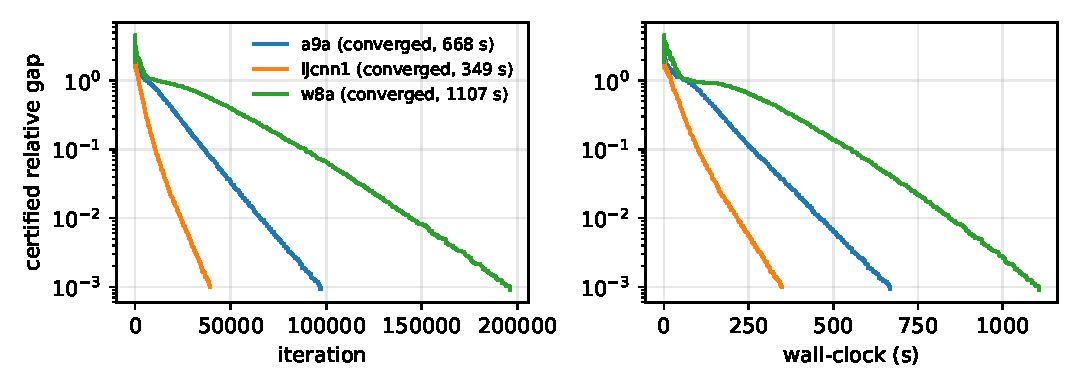
\includegraphics[width=.8\linewidth]{figs/fig_realdata_trace.pdf}
\caption{Certified relative gap of ETA on a9a and w8a ($L_2$, $C=0.1$,
uncapped), versus iteration and wall-clock: linear-rate convergence in
the dense-support regime, at $O(n^2)$-type cost.}\label{fig:trace}
\end{figure}

\paragraph{Hardware and concurrency.} One dedicated 32-vCPU Intel Xeon
2.6\,GHz Lightning Studio, 122\,GB RAM, Linux, Python 3.12, NumPy 2.4
with OpenBLAS 0.3.31, \texttt{OMP\_NUM\_THREADS=1}; the $L_2$ battery
ran 14 cells and the regime battery 12 cells concurrently (the gisette,
covtype and w8a $C{=}10$ cells of Table~\ref{tab:l2} were completed in
later passes with 11--14 workers and no other load). The uncapped
a9a/w8a runs in Figure~\ref{fig:trace} were made earlier on the same
machine under a different load (LIBLINEAR took $12$ and $48$\,s there
against $4$ and $23$\,s in the capped battery), so ratios across the two
runs carry a factor of roughly two of uncertainty; ratios within a
battery do not.

\paragraph{Reference solver in the KL2 cells.} The hinge-loss
\texttt{SVC(rbf, C=1)}, a different objective, took $8.6\pm2.9$ (a9a),
$3.4\pm0.3$ (covtype), $83.5\pm13.1$ (gisette), $1.1\pm0.0$ (ijcnn1) and
$4.9\pm1.2$\,s (w8a), with test accuracies $0.789$, $0.783$, $0.977$,
$0.950$ and $0.975$, within one point of the $L_2$ solutions and on
either side of them.

\paragraph{Step ablation, blocks and shrinking (synthetic).} Iteration
counts at $\varepsilon=10^{-6}$ (single instances): $d{=}30$, $n{=}200$:
toward $158{,}941$, midpoint $148{,}996$, away $106$, pairwise $181$;
$d{=}100$, $n{=}1{,}000$: toward and midpoint fail within $300{,}000$,
away $15{,}886$, pairwise $3{,}921$. At the working tolerance $10^{-3}$
the pairwise/away gain over the midpoint heuristic is only $\sim\!11\%$,
which is why the heuristic sufficed in \cite{gupta2026}. Block transfers
cut iterations $4$--$30\times$ relative to single MDM (e.g.\
$43{,}486\to1{,}551$ on a dense-support $L_2$ instance at $d{=}1{,}000$)
and are the only configuration that reaches the certified tolerance on
MNIST odd-vs-even. Figure~\ref{fig:shrink} shows the screening
speed-ups and Figure~\ref{fig:final} the consolidated comparison: hard
margins $0.24$ vs LIBSVM's $0.39$\,s at $d{=}1{,}000$ and $8.6$ vs
$20.5$\,s at $d{=}10{,}000$; $0.21$ vs $0.42$\,s at
$\varepsilon{=}10^{-5}$ (where the paper-style configuration fails to
converge); RBF hard margin $0.76$ vs $1.28$\,s; $\nu$-SVM $18.5$ vs
$21.9$\,s; synthetic $L_2$ ($d{=}1{,}000$, $C{=}1$) $8.9$ vs
LIBLINEAR's $13.8$\,s; MNIST odd-vs-even $82.8$ vs LIBLINEAR's
$55.0$\,s. Distances agree within tolerance on every row.

\begin{table}[h]\centering\scriptsize
\caption{Two-sided schedules on the synthetic instances of this appendix ($n{=}5{,}000$ per class, $k{=}16$): the unconditional $V$-then-$W$ order used for the batteries versus the schedule of Lemma~\ref{lem:twosided} (larger-gap side first, second side skipped after a drop). Drop steps and skipped second-side steps are counted over the run.}\label{tab:sched}
\begin{tabular}{lllrrrr}\toprule
instance & schedule & time (s) & iterations & drops & skips & distance \\\midrule
hard margin, $d{=}1000$, $\varepsilon{=}10^{-5}$ & unconditional & 0.1 & 16 & 0 & 0 & 55.339365 \\
hard margin, $d{=}1000$, $\varepsilon{=}10^{-5}$ & Lemma~\ref{lem:twosided} & 0.2 & 16 & 0 & 0 & 55.339365 \\
\midrule
$L_2$ overlap, $d{=}100$, $C{=}1$ & unconditional & 7.9 & 11,216 & 638 & 0 & 0.078400 \\
$L_2$ overlap, $d{=}100$, $C{=}1$ & Lemma~\ref{lem:twosided} & 8.1 & 10,701 & 599 & 316 & 0.078400 \\
\midrule
$L_2$ overlap, $d{=}1000$, $C{=}1$ & unconditional & 4.3 & 2,951 & 172 & 0 & 0.578143 \\
$L_2$ overlap, $d{=}1000$, $C{=}1$ & Lemma~\ref{lem:twosided} & 4.3 & 3,001 & 180 & 121 & 0.578143 \\
\bottomrule
\end{tabular}\end{table}

\begin{table}[h]\centering\scriptsize
\caption{Block-size ablation on the same instances (current code): single MDM ($k{=}1$) versus blocks of $k$ transfers. Iterations fall with $k$; wall-clock does not fall in proportion, because each block iteration touches more columns.}\label{tab:kabl}
\begin{tabular}{lrrrrr}\toprule
instance & $k$ & time (s) & iterations & columns & drops \\\midrule
hard margin, $d{=}1000$, $\varepsilon{=}10^{-5}$ & 1 & 0.3 & 296 & 104 & 0 \\
hard margin, $d{=}1000$, $\varepsilon{=}10^{-5}$ & 4 & 0.2 & 36 & 103 & 0 \\
hard margin, $d{=}1000$, $\varepsilon{=}10^{-5}$ & 16 & 0.2 & 16 & 103 & 0 \\
hard margin, $d{=}1000$, $\varepsilon{=}10^{-5}$ & 32 & 0.2 & 16 & 109 & 0 \\
\midrule
$L_2$ overlap, $d{=}100$, $C{=}1$ & 1 & 10.7 & 75,021 & 1,343 & 0 \\
$L_2$ overlap, $d{=}100$, $C{=}1$ & 4 & 11.2 & 24,606 & 1,632 & 416 \\
$L_2$ overlap, $d{=}100$, $C{=}1$ & 16 & 9.0 & 10,701 & 2,404 & 599 \\
$L_2$ overlap, $d{=}100$, $C{=}1$ & 32 & 10.4 & 7,606 & 3,076 & 305 \\
\midrule
$L_2$ overlap, $d{=}1000$, $C{=}1$ & 1 & 12.2 & 43,521 & 1,251 & 0 \\
$L_2$ overlap, $d{=}1000$, $C{=}1$ & 4 & 6.7 & 10,071 & 1,330 & 177 \\
$L_2$ overlap, $d{=}1000$, $C{=}1$ & 16 & 4.3 & 3,001 & 1,348 & 180 \\
$L_2$ overlap, $d{=}1000$, $C{=}1$ & 32 & 4.6 & 1,741 & 1,396 & 170 \\
\bottomrule
\end{tabular}\end{table}


\begin{figure}[h]\centering
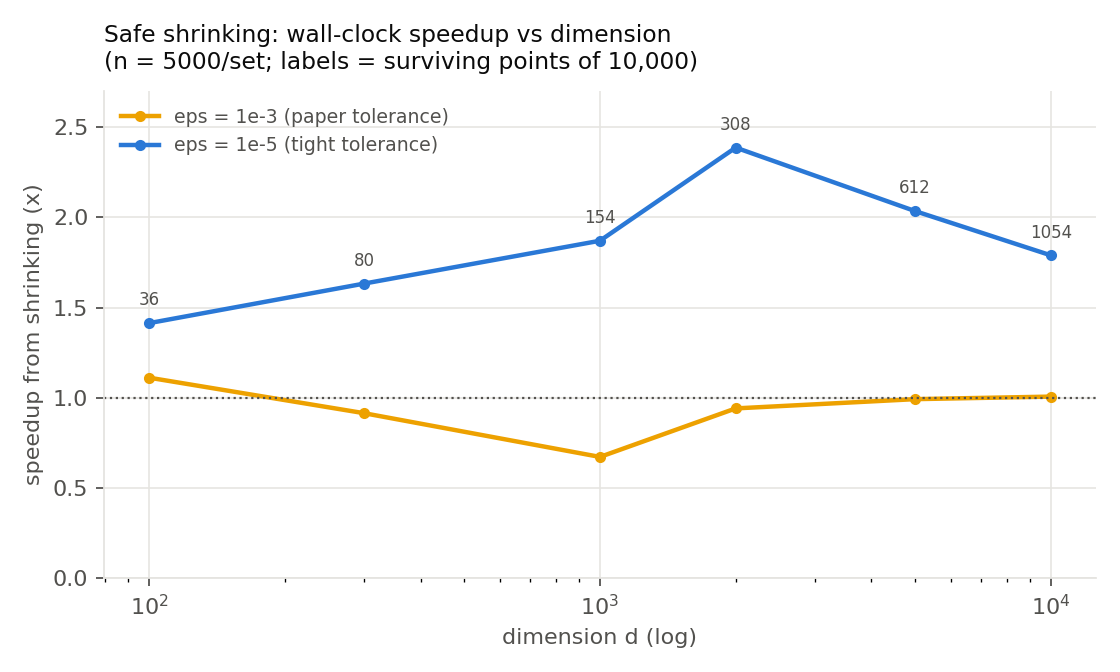
\includegraphics[width=.7\linewidth]{figs/fig_shrink.png}
\caption{Safe screening: wall-clock speed-up vs dimension at two
tolerances on the separated synthetic protocol; labels are surviving
points of $10{,}000$.}\label{fig:shrink}
\end{figure}

\begin{figure}[h]\centering
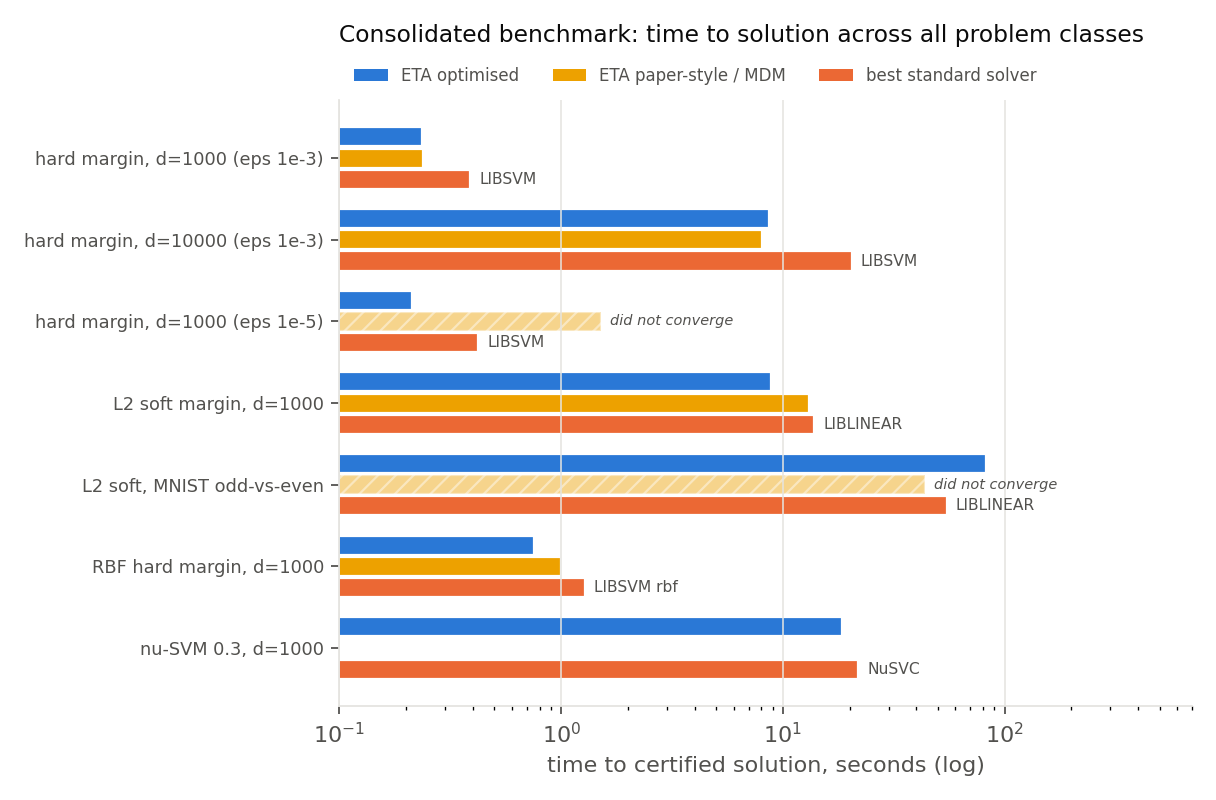
\includegraphics[width=.78\linewidth]{figs/fig_final.png}
\caption{Time to certified solution on seven problem classes: optimised
ETA vs the paper-style configuration vs the best standard solver per
class.}\label{fig:final}
\end{figure}

\section{Extended related work}\label{app:related}
\paragraph{Swap steps.} Blended pairwise conditional gradients
\cite{tsuji2022} also remove pairwise FW's swap-step bound with a guard,
there between the pairwise step and a FW step, and \cite{rinaldi2023}
avoid bad steps with a short-step chain. Our guard compares an
aggregated block of $k$ transfers with the single MDM step and falls
back to an away step, so the drop-step count of away-step FW applies
unchanged. Block-coordinate FW \cite{lacoste2013bcfw} blocks over
\emph{coordinates} of a product domain rather than aggregating pairs on
one polytope.
\paragraph{Screening and identification.} Gap-safe rules
\cite{ndiaye2017,shibagaki2016} screen with a radius from the duality
gap and identify the support in finite time; the active-set complexity
of away-step FW \cite{bomze2020} and the strict-complementarity bounds
of \cite{garber2020} give the same identification from the algorithm's
side. Theorem~\ref{thm:activation} is the polytope-distance instance,
with constants tied to the TA certificate; the SVM rules of
\cite{elghaoui2012,ogawa2013} are its ancestors.
\paragraph{Synthetic results in brief.} Away and pairwise steps
converge at $\varepsilon=10^{-6}$ where the toward and midpoint steps of
\cite{gupta2026} do not. Screening reduces $10{,}000$ points to
$36$--$1{,}054$ survivors at $\varepsilon=10^{-5}$. On seven synthetic
and small-real problem classes the optimised solver is fastest to a
certified solution on six ($1.6$--$2.5\times$ ahead of LIBSVM,
LIBLINEAR or NuSVC); the exception, MNIST odd-vs-even, is a
dense-support $L_2$ problem. On the four classes where single MDM also
converges, blocks and guard add only $0.9$--$1.5\times$ in wall-clock;
their clear wins are the two classes (tight tolerance, MNIST) where
single MDM does not converge at all.

\section{Numerical verification of the analysis}\label{app:num}
Lemma~\ref{lem:block} was checked on $4{,}000$ random ensembles
including heavily clipped and boundary cases (worst slack at machine
precision); Proposition~\ref{prop:orth} on $500$ near-orthogonal
ensembles; Lemma~\ref{lem:gapid} to $10^{-9}$ at arbitrary iterates;
Lemma~\ref{lem:twosided} on instrumented two-sided runs (no drop
iteration added a support index, and every non-drop iteration met the
gain bound with $M$ replaced by the computable upper bound
$\operatorname{diam}V+\operatorname{diam}W$); and Theorem~\ref{thm:activation} on instances whose optimal
face was computed by an exact QP: at every activating round all
zero-weight non-face points were screened, and the final working set
equalled the optimal face exactly. Over $5{,}000$ instrumented live
block steps none increased the objective. All checks are test files in
the released code.

\end{document}
